\subsection{Artifically Intelligent Agents}
    It is generally accepted that an artificial intelligence needs to possess the qualities shown in Figure \ref{fig:AIcapabilities} \cite{Russell2010-wv,Nilsson2009-rp,Luger2008-vf}\footnote{This group of capabilities would generally be accepted in the AI community, although it may be necessary to add other categories like imagination, creativity, and social interaction. Of course this set of attributes is not universally accepted, and is still being refined.}. However, the following simple definitions will help to ground further discussion in the paper:

    \begin{description}
        \item [Reasoning (R)]: The ability to solve problems, and make conclusions.
        \item [Knowledge Representation (K)]: The ability to internally represent knowledge of information that has been learned.
        \item [Planning (Pl)]: The ability to make a plan in order to accomplish a goal within an environment.
        \item [Learning (L)]: The ability to learn from experience and data.
        \item [Perception (Pe)]: The ability to use different sensors to perceive the surrounding environment.
        \item [Motion/Manipulation (M)]: The ability to move within an environment and manipulate parts of it.
        \item [Interaction (I)]: The ability to interact with other intelligent agents. For communicating with humans this could involve some type of natural language interface.
    \end{description}

	\begin{figure}[htbp]
    	\centering
     	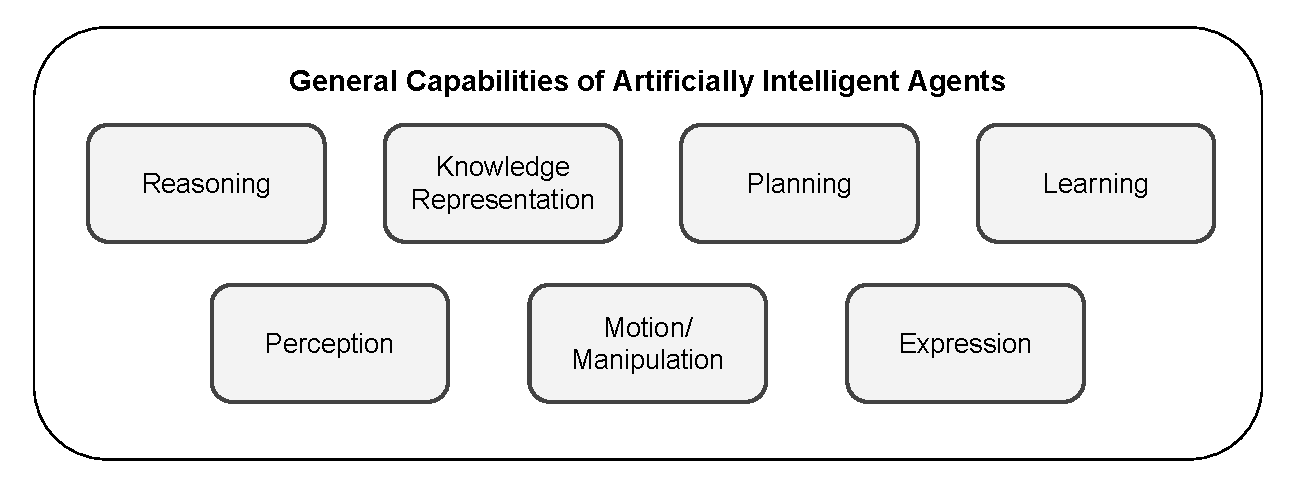
\includegraphics[width=0.7\textwidth]{Figures/AI_capabilities}
    	\caption{List of the capabilities of an artificial general intelligence. In this paper an AI is defined as a system that possesses at least one of the capabilities illustrated.}
        \label{fig:AIcapabilities}
    \end{figure}

    As noted by \cite{Tripp2011-cq} technology spans a wide spectrum of capabilities. With regards to autonomous systems one might consider anything from a thermostat, to a Tesla autopilot. While most of the current focus is geared towards our capability to trust `advanced' technology, for the purposes of this survey I wish to take a more holistic view and use the term Artificially Intelligent Agent (AIA) to encompass a broad range of technologies that can be considered automatic by some sense of the word. \nisarcomm{need to reconcile with earlier disclaimer on restricting your attention, e.g. to ignore things like gain/phase margin}

    It should be noted that the categories are not clearly separable; for instance where does the capability to plan end, and reasoning begin? Similar questions could be asked of the other capabilities. Regardless, given this set of capabilities an AIA can then be defined as:
    
    \begin{description}
    	\item [***Note***:] add a bit more, there is probably an assumption about some purpose or goal
        \item[Artificially Intelligent Agent:] an agent that possess, to some extent, at least one of the capabilities shown in the figure \ref{fig:AIcapabilities}. 
    \end{description}

    Of course, with such a broad definition, there will also be a broad range of different AIAs. \edit{It is argued here that it is most useful} to classify that range along two axes: adaptability, and capability. \nisarcomm{What do you mean by `adaptability'? What do you mean by `capability'?} In the AI community Low adaptability has been termed `narrow' and high adaptability has been termed `broad'. Similarly, low capability has been termed `weak' and high capability `strong'. Figure \ref{fig:StrongWeak} is a depiction of these two axes, and where some typical AIAs might fall in that space.

	\begin{figure}[htbp]
    	\centering
     	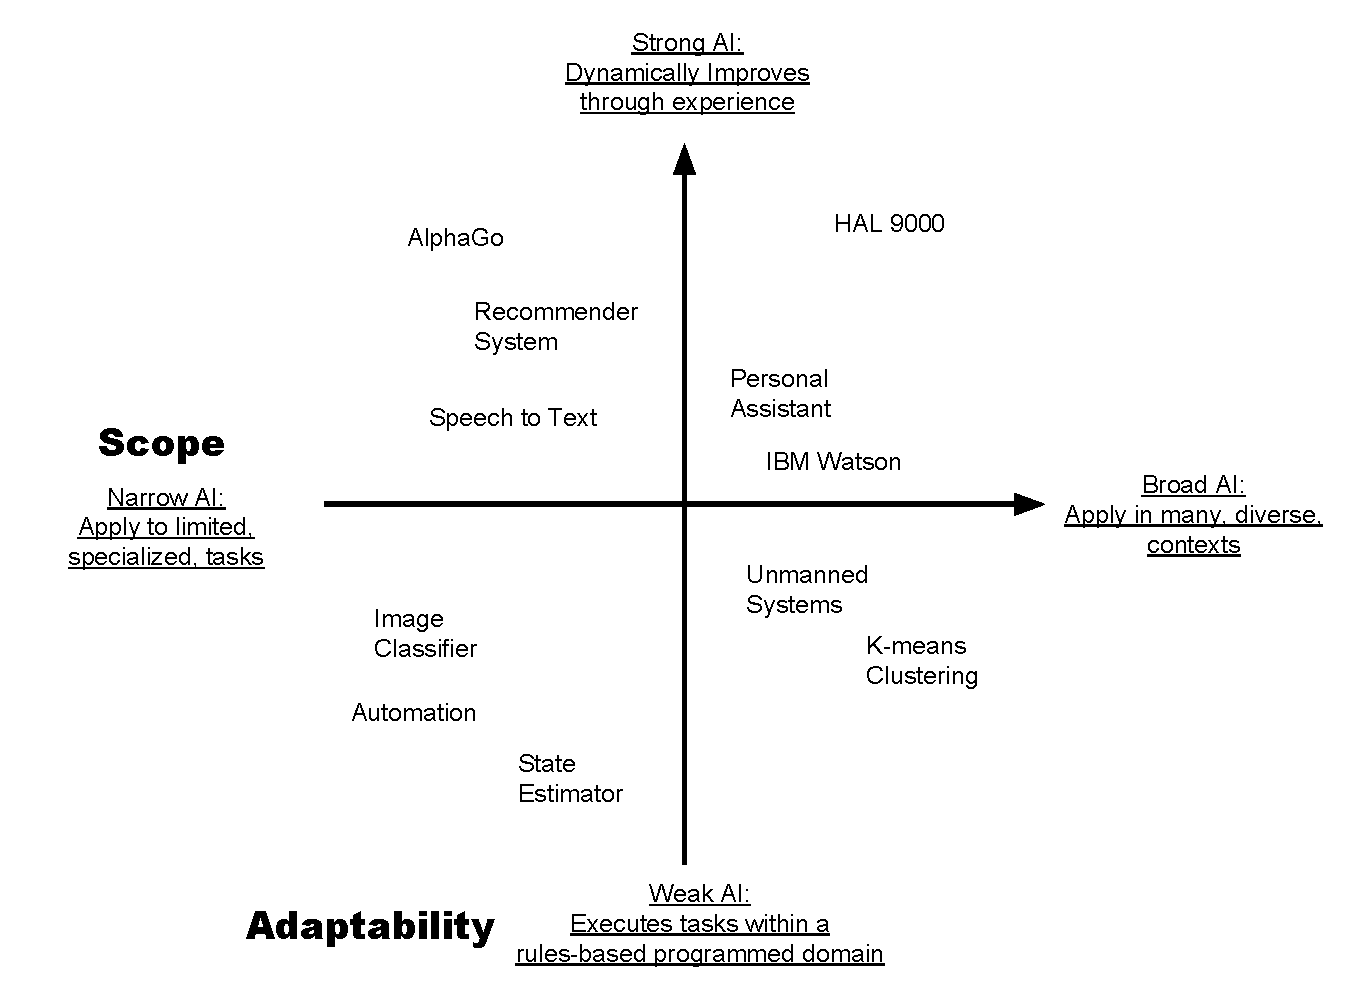
\includegraphics[width=0.9\textwidth]{Figures/strong_weak_narrow_broad.pdf}
    	\caption{Illustration of the range of systems encompassed by the AIA definition. Horizontal axis reflects the scope of the AIA, the vertical axis reflects the adaptability of the AIA.}
        \label{fig:StrongWeak}
    \end{figure}

    To make sure the point is clear, the research discipline called machine learning (ML) is a subset of the AI research landscape. Individual ML algorithms might be thought of as being a narrowly scoped AI that is contained within only one of the AIA capabilities. \nisarcomm{Next sentence is a non-sequitur -- seems to be missing a transition to next list.} Concretely, the following systems currently exist and may possess the listed AIA capabilities.

    \begin{enumerate}
         \item An autonomous bottle capping machine might \textbf{perceive} bottles, and \textbf{manipulates} parts to place caps on them
         \item An unmanned aerial system (UAS) might possess the ability to \textbf{plan} missions, \textbf{perceive} its location, and execute \textbf{motion} of its components to carry out a plan
         \item A virtual personal assistant might be capable of \textbf{interacting} with a user, \textbf{learn} the user's preferences, and \textbf{reason} about what assistance the user needs
         \item An image classifier might possess the capability to \textbf{learn} image classes from labeled examples and predict the class of never-before-seen new images.
     \end{enumerate}

\nisarcomm{Remove first person voice}    Arguably I might just use the term artificial intelligence (AI) instead of AIA, however the term AI carries too much ambiguity (in its fullest meaning it would possess all capabilities from figure \ref{fig:AIcapabilities}, and more). Using AIA allows me to broadly include \emph{any} system in the adaptability/capability plane. Figure \ref{fig:StrongWeak} shows some examples of AIAs and their places on the plane.

    One might also question the need to define AIAs in the first place. This is to aid in the search \edit{for and understanding of} assurances. As will be shown later, assurances span the range of AIAs \nisarcomm{not sure what `assurances span the range of AIAs' means -- assurances are features of AIAs, not AIAs themselves...}, so that an automation system \edit{such as a ...} might be able to use similar assurances \edit{(or more generally, similar principles of assurance) as might} a self-driving car, and vice-versa.

    This definition, while broad, is still useful because it encompasses many of the systems that are typically described %currently being marketed (you're not in business school)
    as ``artificially intelligent''. More importantly, many of the assurances that exist for the simplest AIAs (e.g. a simple k-means classifier) can be extended for use in more advanced AIAs. In other words, the definition of AIAs sets an appropriate scope for the bodies of research that are likely to contain assurances and assurance principles that \edit{can be generalized/extended} to any intelligent computing system. The definition of AIAs and their range of capabilities also helps to understand and establish what kinds of assurances might be needed \edit{in future systems}. For example assurances from an AIA that can only carry out planning tasks will probably differ in design and/or application from assurances from an AIA that can \edit{only} carry out perception tasks. 
